\chapter{Overview of the search of \texorpdfstring{\hmm}{H to muons} decay at CMS}
% Need to use \textorpdfstring{} so it also shows in pdf bookmarks 

In 2012, a new boson at 125 \GeV was discovered by ATLAS and CMS at the LHC~\cite{Aad:2012tfa, Chatrchyan:2012xdj, Chatrchyan:2013lba}. 
Various measurements have been performed to probe the properties of this boson ever since, 
and the boson was later ackownledged as the Higgs boson predicted by the SM.
Up to now, the couplings between the Higgs boson and the electroweak gauge bosons have been observed to be consistent with the SM prediction, 
while the Yukawa couplings between the Higgs boson and the fermions have only been established for the third generation fermions. 
The first and second generation fermions have less mass than their third generation counterparts and thus weaker coupling to the Higgs boson, 
as the coupling strength is proportional to the mass of the fermion.
This leads to significantly smaller branching fractions of the decay modes of the Higgs boson to the first or second generation fermions, 
and poses a substantial challenge to the searches for such decays.  
The \hmm decay in particular, has a branching raio of ${\brhmm = 2.18 \times 10^{-4}}$, 
which corresponds to an expectation of about 1000 event instances recorded by CMS during the Run 2 data-taking period of the LHC (year 2016 to 2018).
In contrast, these 1000 so-called signal events are engulfed by millions of events produced through other processes (background events) that mimic their experimental signitures.
The search for the \hmm decay, in a nutshell, is a struggle to make the signal events stand out from the vast backgrounds with statistical significance.

The search for the \hmm decay has been conducted using proton-proton (pp) collision data collected at center-of-mass energies of 7, 8, and 13 \TeV
by the CMS Collaboration~\cite{2015184, PhysRevLett.122.021801} and the ATLAS Collaboration~\cite{201468, PhysRevLett.119.051802, Aad:2020xfq}.
The latest result~\cite{PhysRevLett.122.021801} from CMS prior to this work reported an observed (expect in absence of \hmm decay) upper limit of 2.9 (2.2) times the 
SM prediction of the Higgs boson production and the \brhmm, at the 95\% confidence level (CL).
More details of this previous result can also be found in the PhD thesis of Andrew Carnes~\cite{carnesthesis}.  

Aside from the challenging nature of the \hmm analysis, many efforts can be made to improve the separation of the signal and the backgrounds, 
allowing for a sizable refinement of the result.
First of all, the Higgs boson has a narrow natural width, and the muons are well identified objects in the CMS detector.
This means that the two muons from the Higgs decay always compose an invariate mass near the nominal Higgs mass, 125 \GeV.
While for the background, the two muons for most times come from the decay of a \PZ boson, 
or sometimes come from the decay of two different particles, for example a \Pqt and \Paqt quark pair.
The \PZ boson has a mean mass at 91.2 \GeV and a natural width of 2.5 \GeV, making a slowly falling tail in the mass spectrum around 125 \GeV.
For the muons that come from two different sources, their invariant mass follows a flat random distribution near the mass range of interest.
Therefore, the signal can be strongly distinguished against the background in the dimuon invariant mass spectrum, 
as a sharpe peak against a smooth falling shape. Figure~\ref{fig:dimuon_mass_shapes} shows the conceptual shape of these mass spectra. 
\begin{figure}[!htb]
    \centering
    \captionsetup{justification=justified}
    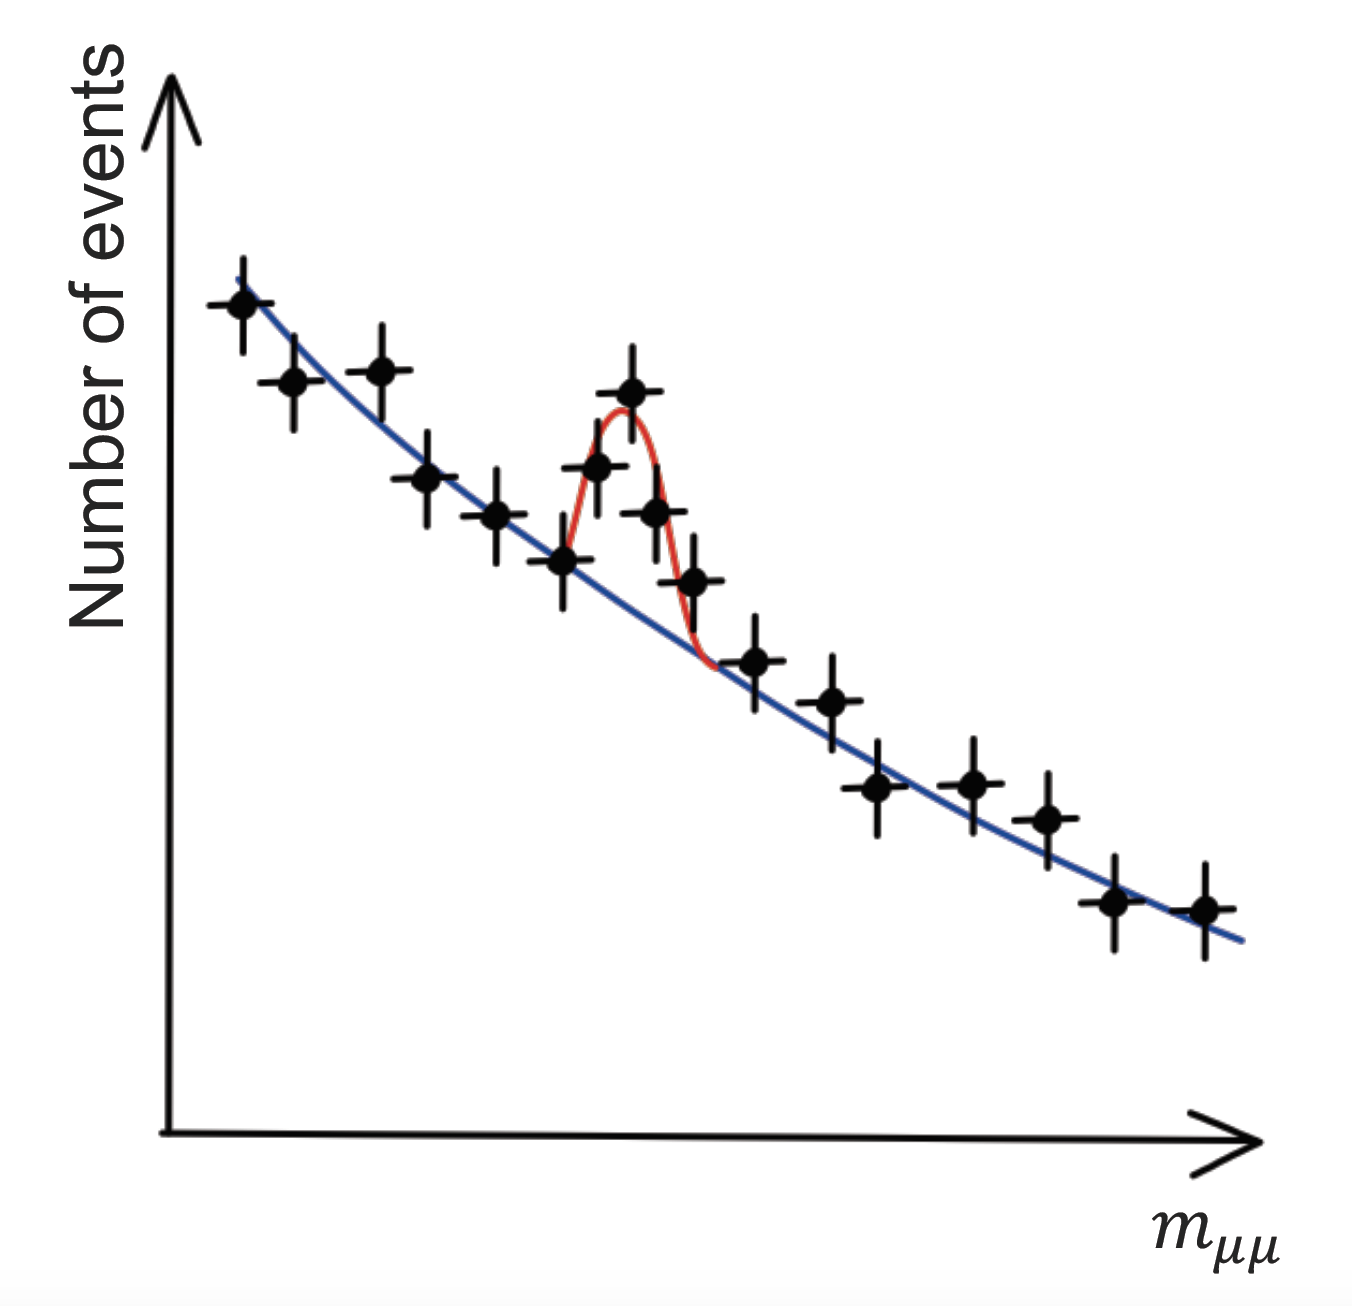
\includegraphics[width=0.6\textwidth]{pics/hmm_mass_sketch.png}
    \caption{A conceptual plot for the dimuon mass shapes for the signal and the background. 
             The blue line shows the expected background shape, while the red line shows the expected signal shape on top of it.}
    \label{fig:dimuon_mass_shapes}
\end{figure}

Furthermore, the Higgs boson is produced via several distinct production modes, each with some unique kinematic characteristics. 
By applying selection criteria targeting a certain signal production mode, it is possible to select a specific part of the kinematic phasespace that is enriched with that signal, 
and reject many background processes that do not share the same kinematic features. 
There are four main production modes considered in this analysis, ordered by cross section: the gluon fusion (\ggH), the vector boson fusion (\qqH or qqH), 
the associated production with a weak vector boson (\VH), and the associated production with a pair of top quarks (\ttH). 
The feynman diagrams for these main production modes are shown in Figure~\ref{fig:main_higgs_modes}.
Some other minor production modes are also considered as signal contributions, including the associated production with a pair of bottom quarks (\bbH),
the associated production with a \PZ boson through gluon fusion (\ggZH), the associated production with a top quark and a \PW boson (\tHW), 
and the associated production with a top quark and a light quark (\tHq). 
The feynman diagrams for these minor production modes are shown in Figure~\ref{fig:minor_higgs_modes}.
Table~\ref{tab:signal_xsec} summarizes the cross section for all these production modes, 
along with the expected number of events in the Run 2 dataset (137 \invfb).

\begin{figure}[!htb]
    \centering 
    \captionsetup{justification=centering}
    \begin{subfigure}[b]{0.45\textwidth} % b for bottom alignment so caption is at the same height
        \centering
        \feynmandiagram[horizontal=g1 to t1, horizontal=t2 to h] {
            g1 [particle = \Pg] -- [gluon] t1,
            t1 -- [fermion, edge label = \Pqt] t2 -- [fermion, edge label = \Pqt] t3 -- [fermion, edge label = \Pqt] t1,
            g2 [particle = \Pg] -- [gluon] t3,
            t2 -- [scalar] h [particle = \PH],
            g1 -- [draw=none] g2,
        };

        \caption*{\ggH}
    \end{subfigure} 
    %to put these two diagrams side by side. no empty line in between these two blocks, otherwise it indicates an empty line in the pdf
    \begin{subfigure}[b]{0.45\textwidth}
        \centering
        \feynmandiagram[horizontal=b to h]{
            q1 [particle = $\Pq_{1}$] -- [fermion] a -- [fermion] aq1 [particle = $\Pq^\prime_{1}$],
            a -- [boson, edge label = \PV] b -- [boson, edge label = \PV] c,
            b -- [scalar] h [particle = \PH],
            aq2 [particle = $\Pq_{2}$] -- [fermion] c -- [fermion] q2 [particle = $\Pq^\prime_{2}$],

            q1 -- [draw = none] n -- [draw = none] aq2,
            a -- [draw = none] c,
            aq1 -- [draw = none] h -- [draw = none] q2,

        };
        \caption*{\qqH}
    \end{subfigure}

    \begin{subfigure}[b]{0.45\textwidth}
        \centering
        \feynmandiagram[horizontal=a to b] {
            q [particle = \Pq] -- [fermion] a -- [anti fermion] aq [particle = $\Pq^\prime$],
            a -- [boson, edge label = \PV] b,
            v [particle = \PV] -- [boson] b -- [scalar] h [particle = \PH],
        };
        \caption*{\VH}
    \end{subfigure}
    \begin{subfigure}[b]{0.45\textwidth}
        \centering
        \feynmandiagram[horizontal=b to h]{
            g1 [particle = \Pg] -- [gluon] a -- [fermion] t1 [particle = \Pqt],
            a -- [anti fermion, edge label = \Paqt] b -- [anti fermion, edge label = \Pqt] c,
            b -- [scalar] h [particle = \PH],
            g2 [particle = \Pg] -- [gluon] c -- [anti fermion] t2 [particle = \Paqt],

            g1 -- [draw = none] n -- [draw = none] g2,
            a -- [draw = none] c,
            t1 -- [draw = none] h -- [draw = none] t2,
        };
        \caption*{\ttH}
    \end{subfigure}
    \caption{Main production modes of the Higgs boson.}
    \label{fig:main_higgs_modes}
\end{figure}



\begin{figure*}[!htb]
    \centering
    \captionsetup{justification=centering}
    \begin{subfigure}[b]{0.45\textwidth}
        \centering
        \feynmandiagram[horizontal=b to h]{
            g1 [particle = \Pg] -- [gluon] a -- [fermion] b1 [particle = \Pqb],
            a -- [anti fermion, edge label = \Paqb] b -- [anti fermion, edge label = \Pqb] c,
            b -- [scalar] h [particle = \PH],
            g2 [particle = \Pg] -- [gluon] c -- [anti fermion] b2 [particle = \Paqb],

            g1 -- [draw = none] n -- [draw = none] g2,
            a -- [draw = none] c,
            b1 -- [draw = none] h -- [draw = none] b2,
        };
        \caption*{\bbH}
    \end{subfigure}
    \begin{subfigure}[b]{0.45\textwidth}
        \centering
        \feynmandiagram[horizontal=a to b] {
            g [particle = \Pg] -- [gluon] a -- [anti fermion] qb [particle = \Pqb],
            a -- [fermion, edge label = \Pqb] b,
            w [particle = $\PW^{-}$] -- [boson] b -- [fermion, edge label = \Pqt] th -- [fermion] t [particle = \Pqt],
            th -- [scalar] h [particle = \PH],
            t -- [draw = none] h -- [draw = none] w, 
        };
        \caption*{\tHW}
    \end{subfigure}

    \begin{subfigure}[b]{0.45\textwidth}
        \centering
        \feynmandiagram[vertical=a to b] {
            q [particle = \Pq] -- [fermion] a -- [fermion] aq [particle = \Paq'],
            a -- [boson, edge label = \PW] b,
            qb [particle = \Pqb] -- [fermion] b -- [fermion, edge label = \Pqt] c,
            c -- [scalar] h [particle = \PH],
            c -- [fermion] t [particle = \Pqt],
            q -- [draw = none] n -- [draw = none] qb,
            aq -- [draw = none] h -- [draw = none] c,
            aq -- [draw = none] h -- [draw = none] t,
        };
        \caption*{\tHq}
    \end{subfigure}
    \begin{subfigure}[b]{0.45\textwidth}
        \centering
        \feynmandiagram[horizontal=b to h]{
            q1 [particle = \Pq] -- [fermion] a -- [fermion] q2 [particle = $\Pq^\prime$],
            a -- [boson, edge label = \PW] b -- [boson, edge label = \PW] c,
            b -- [scalar] h [particle = \PH],
            qb [particle = \Pqb] -- [fermion] c -- [fermion] qt [particle = \Pqt],

            q1 -- [draw = none] n -- [draw = none] qb,
            a -- [draw = none] c,
            q2 -- [draw = none] h -- [draw = none] qt,
        };
        \caption*{\tHq}
    \end{subfigure}

    \begin{subfigure}[b]{0.45\textwidth}
        \centering
        \feynmandiagram[horizontal=g1 to q1, horizontal=q2 to z] {
            g1 [particle = \Pg] -- [gluon] q1,
            q1 -- [fermion, edge label' = \Pq] q2 -- [fermion, edge label' = \Pq] q3 -- [fermion, edge label' = \Pq] q1,
            g2 [particle = \Pg] -- [gluon] q3,
            q2 -- [boson, edge label = \PZ] z ,
            z -- [boson] z2 [particle = \PZ],
            z -- [scalar] h [particle = \PH],
            g1 -- [draw=none] g2,
        };
        \caption*{\ggZH}
    \end{subfigure} 
    \begin{subfigure}[b]{0.45\textwidth}
        \centering
        \feynmandiagram[horizontal=t1 to t2] {
            g1 [particle = \Pg] -- [gluon] t1 -- [fermion, edge label = \Pqt] t2 -- [boson] z [particle = \PZ],
            g2 [particle = \Pg] -- [gluon] t4 -- [anti fermion, edge label = \Pqt] t3 -- [scalar] h [particle = \PH],
            t1 -- [anti fermion, edge label = \Pqt] t4,
            t2 -- [fermion, edge label = \Pqt] t3,
            g1 -- [draw = none] g2,
            z -- [draw = none] h,
        };
        \caption*{\ggZH}
    \end{subfigure} 
    \caption{Examples of minor Higgs production modes.}
    \label{fig:minor_higgs_modes}
\end{figure*}

\begin{table}[!htb]
    \centering
    \captionsetup{justification=justified}
    \topcaption{Production modes of the Higgs boson in the pp collision at the LHC, their cross section for $\mh = 125 \GeV$, 
                and the expected number of events for the Run 2 integrated luminosity ($137 \invfb$). 
                The leptons ($\ell$) in the table refer to electrons or muons.}
    \begin{tabular}{lccc}
        \hline
        signal mode         & decay mode                & Cross section (\pb)   & Expected number of events \\
        \hline
        \ggH                & inclusive                 & 48.58                 & 1450 \\
        \qqH                & inclusive                 & 3.782                 & 113 \\
        \WH                 & inclusive                 & 1.373                 & 41.0 \\
                            & $\PW\to\ell\nu$           & 0.293                 & 8.75 \\
%                            & $\PW\to$ hadrons          & 0.926                 & 27.6 \\
        ${\Pq\Pq\to\PZ\PH}$ & inclusive                 & 0.761                 & 22.7 \\
                            & $\PZ\to\ell\ell$          & 0.051                 & 1.53 \\
%                            & $\PZ\to\nu\nu$            & -                     & - \\
%                            & $\PZ\to$ hadrons          & -                     & - \\
        \ggZH               & inclusive                 & 0.123                 & 3.67 \\
                            & $\PZ\to\ell\ell$          & 0.008                 & 0.25 \\
%                            & $\PZ\to\nu\nu$            & -                     & - \\
%                            & $\PZ\to$ hadrons          & -                     & - \\
        \ttH                & inclusive                 & 0.507                 & 15.1 \\
                            & $\geq 1~\Pqt\to$ leptons  & 0.193                 & 5.76 \\
                            & Both $\Pqt\to$ hadrons    & 0.230                 & 6.86 \\
        \hline
        sum of above        & inclusive                 & 55.13                 & 1646 \\
        \hline
        \bbH                & inclusive                 & 0.488                 & 14.6 \\
        \tHq                & inclusive                 & 0.074                 & 2.21 \\
        \tHW                & inclusive                 & 0.015                 & 0.45 \\
        \hline
        sum of all          & inclusive                 & 55.70                 & 1663 \\
        \hline
    \end{tabular}
    \label{tab:signal_xsec}
\end{table}

Four event categories are definited in this analysis targeting each of the four main Higgs production modes:
apart from the requirement of two muons that makes a candidate for a Higgs boson, 
the \ttH category asks for the presence of additional b-jets (from the decay of the top quarks) in the event,
the \VH category asks for the presence of additional leptons (\Pe or \mu, from the decay of the vector boson) in the event, 
the \qqH category asks for two energetic and forward jets in the event,
while the \ggH category does not ask for additional objects and collects all events that are not selected by the other three categories.
No dedicated category is made for the minor signal modes, since they either have very similar features as one of the main modes, 
or have too small cross section to make a difference.

With sush selections, natually, each of the selected phasespaces presents a distinct event topology and contains a distinct composition of background. 
Therefore, the analysis is performed independently in each of the event categories, following different optimized strategies. 
The detailed description of the analysis strategies in each event category is given in Section~\ref{sec:hmm_cat_and_strategy}.

\bigskip
\section{Data and simulation samples}
This analysis uses the proton-proton collision data collected by the CMS detector during Run 2,
which corresponds to a total integrated luminosity of 137.2\invfb.

The triggers used in this analysis are the single muon triggers, which impose some loose isolation requirements and a \pt threshold on the HLT muon candidates.
The \pt cut is 27 (24) \GeV for data collected in 2017 (2016, 2018). 
For the muons selected in this analysis, as explained in Section~\ref{sec:obj_sel}, the efficiency of these triggers is above 95\%, 
making the selection efficiency for the events with two muons close to 100\%.
acceptance here or in object selection?

Simulated events from the Monte Carlo (MC) event generatores for the signal and the dominant background processes are used to 
optimized the analysis strategy and assess the systematics uncertainties.
The generated events are processed through a detailed simulation of the CMS detector based on \GEANTfour~\cite{AGOSTINELLI2003250}
and are reconstrcuted with the same algorithms that are used for data.
All MC samples except the electroweak $\PZ+jj$ samples (one of the background processes) use \PYTHIA 8.2~\cite{SJOSTRAND2015159} to model the parton showing (PS), 
hadronization, and the underlying event (UE), while the electroweak $\PZ+jj$ samples use \HERWIGpp and \HERWIGSeven~\cite{Bellm:2015jjp} for the same purpose.
The effect of pileup interactions is modelled by overlaying simulated inelastic pp collisions on the hard-scattering event.\\

\bigskip
\subsection{The simulation of the signal processes}
The \ggH signal process is simulated at next-to-leading order (NLO) acuracy in perturbative QCD, using both the \MGvATNLO v2.4.2~\cite{Alwall:2014hca}
and \POWHEG v2.0~\cite{Nason_2004, Frixione_2007, Alioli:2010xd, Bagnaschi:2011tu} MV event generators. 
The \pt distribution fo the Higgs boson produced via gluon fusion is then reweighted to match the \POWHEG~\textsc{nnlops} prediction~\cite{Hamilton:2013fea,Hamilton:2015nsa}. 
The \qqH, ${\Pq\Pq\to\PV\PH}$, and \ttH processes are simulated with \POWHEG~v2.0~\cite{Nason:2009ai,Luisoni:2013kna,Hartanto:2015uka} at NLO precision in QCD. 
The \bbH process is simulated at NLO precision in QCD with \POWHEG.
the \tHq, and \tHW processes are generated at leading order (LO) with the \MGvATNLO generator.
The \ggZH process is simulated at LO with the \POWHEG generator.
Simulated signal events are generated, for each production mode, at \mh values of 120, 125, 130 \GeV.
A table summarizing the simulation for signals is shown in Table~\ref{tab:sig_samples}.

\begin{table}[!htb]
    \centering
    \captionsetup{justification=centering}
    \topcaption{Summary of the specification for the simulated Higgs signal samples.}
    \resizebox{\textwidth}{!}{\begin{tabular}{lcccc}
        \hline
        Sample                 &Generator (Perturbative order)    &Parton Shower          &Cross section      &Additional corrections\\
        \hline
        \ggH                   &\MGvATNLO (NLO QCD)               &\PYTHIA                &N3LO QCD, NLO EW   &$\pt(\PH)$ from \textsc{nnlops}\\
        \qqH                   &\POWHEG (NLO QCD)                 &\PYTHIA dipole shower  &NNLO QCD, NLO EW   & -\\
        ${\Pq\Pq\to\PV\PH}$    &\POWHEG (NLO QCD)                 &\PYTHIA                &NNLO QCD, NLO EW   & -\\
        \ggZH                  &\POWHEG (LO)                      &\PYTHIA                &NNLO QCD, NLO EW   & -\\
        \ttH                   &\POWHEG (NLO QCD)                 &\PYTHIA                &NLO QCD, NLO EW    & -\\
        \bbH                   &\POWHEG (NLO QCD)                 &\PYTHIA                &NLO QCD            & -\\
        \tHq                   &\MGvATNLO (LO)                    &\PYTHIA                &NLO QCD            & -\\
        \tHW                   &\MGvATNLO (LO)                    &\PYTHIA                &NLO QCD            & -\\
        \hline
    \end{tabular}}
    \label{tab:sig_samples}
\end{table}

Expected signal yields are normalized to the production cross sections and \brhmm values taken from the recommendations of LHC Yellow Report~\cite{deFlorian:2016spz}.
The \ggH production cross section is computed at next-to-next-to-NLO (N3LO) precision in QCD, and at NLO in electroweak (EW) theory~\cite{Anastasiou:2016cez}. 
The cross section of Higgs boson production in the VBF~\cite{Cacciari:2015jma} and ${\Pq\Pq\to\PV\PH}$~\cite{Brein:2003wg} modes is calculated at next-to-NLO (NNLO) in QCD, 
including NLO EW corrections, while the \ttH cross section is computed at NLO in QCD and EW theory~\cite{Dawson:2003zu,Frixione:2014qaa}. 
The \bbH, \tHq, and \tHW cross sections are computed at NLO in QCD without including higher-order EW corrections~\cite{deFlorian:2016spz,Demartin:2015uha,Demartin:2016axk}. 
The \hmm partial width is computed with \textsc{hdecay}~\cite{Djouadi:1997yw,Spira:1997dg} at NLO in QCD and EW theory.

\bigskip
\subsection{The simulation of the background processes}
The background is modeled consibering various SM processes, summarized in table~\ref{tab:bkg_samples}.
The main background in the \ggH and \qqH categories is the DY process, which is simulated at NLO in QCD using the \MGvATNLO generator. 
The corresponding cross section is calculated with \FEWZ~v3.1b2~\cite{Li:2012wna} at NNLO in QCD and NLO accuracy in EW theory. 
The EW production of a $\PZ$ boson in association with two jets ($\PZ+jj$) is an important background in the VBF category. 
This process is simulated at LO using the \MGvATNLO~v2.6.5 generator. 
The $\PW\PZ$, ${\Pq\Paq\to\PZ\PZ}$, and $\PW\PW$ processes, which constitute the main backgrounds in the $\PV\PH$ category, 
are simulated at NLO in QCD using either the \POWHEG or \MGvATNLO generators. 
Their production cross sections are corrected with the NNLO/NLO $K$ factors taken from Refs.~\cite{Grazzini:2017ckn},~\cite{Grazzini:2015hta}, and~\cite{Gehrmann:2014fva}. 
The gluon-initiated loop-induced ZZ process (\ggZZ) is simulated with the \MCFM~v7.0 generator~\cite{Campbell:2011bn} at LO 
and the corresponding production cross section is corrected to match higher-order QCD predictions, following the strategy detailed in Ref.~\cite{Sirunyan:2017exp}. 
Minor contributions from triboson processes ($\PW\PW\PW$, $\PW\PW\PZ$, $\PW\PZ\PZ$, and $\PZ\PZ\PZ$) are also taken into account and are simulated at NLO in QCD using the \MGvATNLO generator. 
The main backgrounds in the \ttH category involve the production of top quarks. 
The $\Pqt\Paqt$ background is simulated with NLO precision in QCD using the \POWHEG generator, and its cross section is obtained from the \textsc{top++}~v2.0~\cite{Czakon:2011xx} prediction 
that includes NNLO corrections in QCD and resummation of NNLL soft gluon terms. 
The single top quark processes are simulated at NLO in QCD via either \POWHEG or \MGvATNLO and their cross sections are computed, 
at the same order of precision, using \textsc{hathor}~\cite{Kant:2014oha}. 
Finally, contributions from the $\Pqt\Paqt\PZ$, $\Pqt\Paqt\PW$, $\Pqt\Paqt\PW\PW$, ${\Pqt\Paqt\Pqt\Paqt}$, and \tZq processes 
are also considered and are simulated using the \MGvATNLO generator at NLO precision in QCD. 
For the simulated samples corresponding to the 2016 (2017--2018) data-taking periods, the NNPDF~v3.0~(v3.1) NLO (NNLO) parton distribution functions (PDFs) are used~\cite{Ball:2014uwa,Ball:2017nwa}. 
For processes simulated at NLO (LO) in QCD with the \MGvATNLO generator, events from the matrix element (ME) characterized by different parton multiplicities are merged via the FxFx (MLM) prescription~\cite{Alwall:2007fs,Frederix:2012ps}.


\begin{table}[!htb]
    \centering
    \captionsetup{justification=centering}
    \topcaption{Summary of the specification for the simulated background samples.}
    \resizebox{\textwidth}{!}{\begin{tabular}{lcccc}
        \hline
        Sample                              &Generator (Perturbative order)    &Parton Shower          &Cross section      &Additional corrections\\
        \hline
        Drell-Yan                           &\MGvATNLO (NLO QCD)               &\PYTHIA                &NNLO QCD, NLO EW   & -\\
        Zjj-EW                              &\MGvATNLO (LO)                    &\HERWIGpp/\HERWIGSeven &LO                 & -\\
        $\Pqt\Paqt$                         &\POWHEG (NLO QCD)                 &\PYTHIA                &NNLO QCD           & -\\
        Single top quark                    &\POWHEG/\MGvATNLO (NLO QCD)       &\PYTHIA                &NLO QCD            & -\\
        Diboson ($\PV\PV$)                  &\POWHEG/\MGvATNLO (NLO QCD)       &\PYTHIA                &NLO QCD            & NNLO/NLO $K$ factors\\
        \ggZZ                               &\MCFM (LO)                        &\PYTHIA                &LO                 & NNLO/LO $K$ factors\\
        $\Pqt\Paqt\PV$, $\Pqt\Paqt\PV\PV$   &\MGvATNLO (NLO QCD)               &\PYTHIA                &NLO QCD            & -\\
        Triboson ($\PV\PV\PV$)              &\MGvATNLO (LO)                    &\PYTHIA                &NLO QCD            & -\\
        \hline
    \end{tabular}}
    \label{tab:bkg_samples}
\end{table}


\bigskip
\section{Exclusive analyses and their strategies}\label{sec:hmm_cat_and_strategy}
In order to maximally harness the kinematic features in the different production modes of the Higgs boson,
the analysis is conducted in four independent event categories: the \ggH, \qqH, \VH and \ttH categories.
The determination of the event categories is shown in Figure~\ref{fig:event_categories}.
As a common prerequisite in this analysis, all events should contain two opposite-charged (or opposite-sign, OS) muons that makes the candidate for the Higgs boson. 
Then, as a first step, events containing b-tagged jets (either one medium tag or two loose tag of the DeepCSV~\cite{Sirunyan:2017ezt} working points) are classified into the \ttH category.
The \ttH category is further divided into the \ttH leptonic category and the \ttH hadronic category depending on whether the event contains electrons or additional muons (leptonic category), 
or whether it contains at least three jets (hadronic category).
Some events in the \ttH category (containing b-tagged jets) may not pass the secondary selections for neither the leptonic nor hadronic categories.
They are most likely to be background events, and are therefore discarded.
For the events with an absence of b-tagged jets, if they contain additional leptons (electrons or muons), are classified as the \VH category.
Inside the \VH category, events are further tagged as the \WH events if there is one and only one extra lepton in the event, 
or tagged as the \ZH events if there are two same-flavor-opposite-sign (SFOS) extra leptons.
Similar to the case in \ttH category, some events may pass the primary \VH selection but not the secondary \WH or \ZH selections, 
for example an event that contains one extra electron and one extra muon.
Those events are most likely not from the signal processes, and are discarded.
For the events without neither b-tagged jets nor additional leptons, if there are at least two energetic jets, 
composing a jet pair with $\mjj>400\GeV$ and $\detajj>2.5$, the events are tagged as the \qqH events.
Finally, the \ggH category collects all events that are not assigned in the previous steps. 
Most events in the \ggH category are profiled to have either no additional object, or one additional jet.
The detailed definition of the different objects used in this categorization is given in Section~\ref{sec:obj_sel}.

\begin{figure}[!htb]
    \centering
    \captionsetup{justification=justified}
    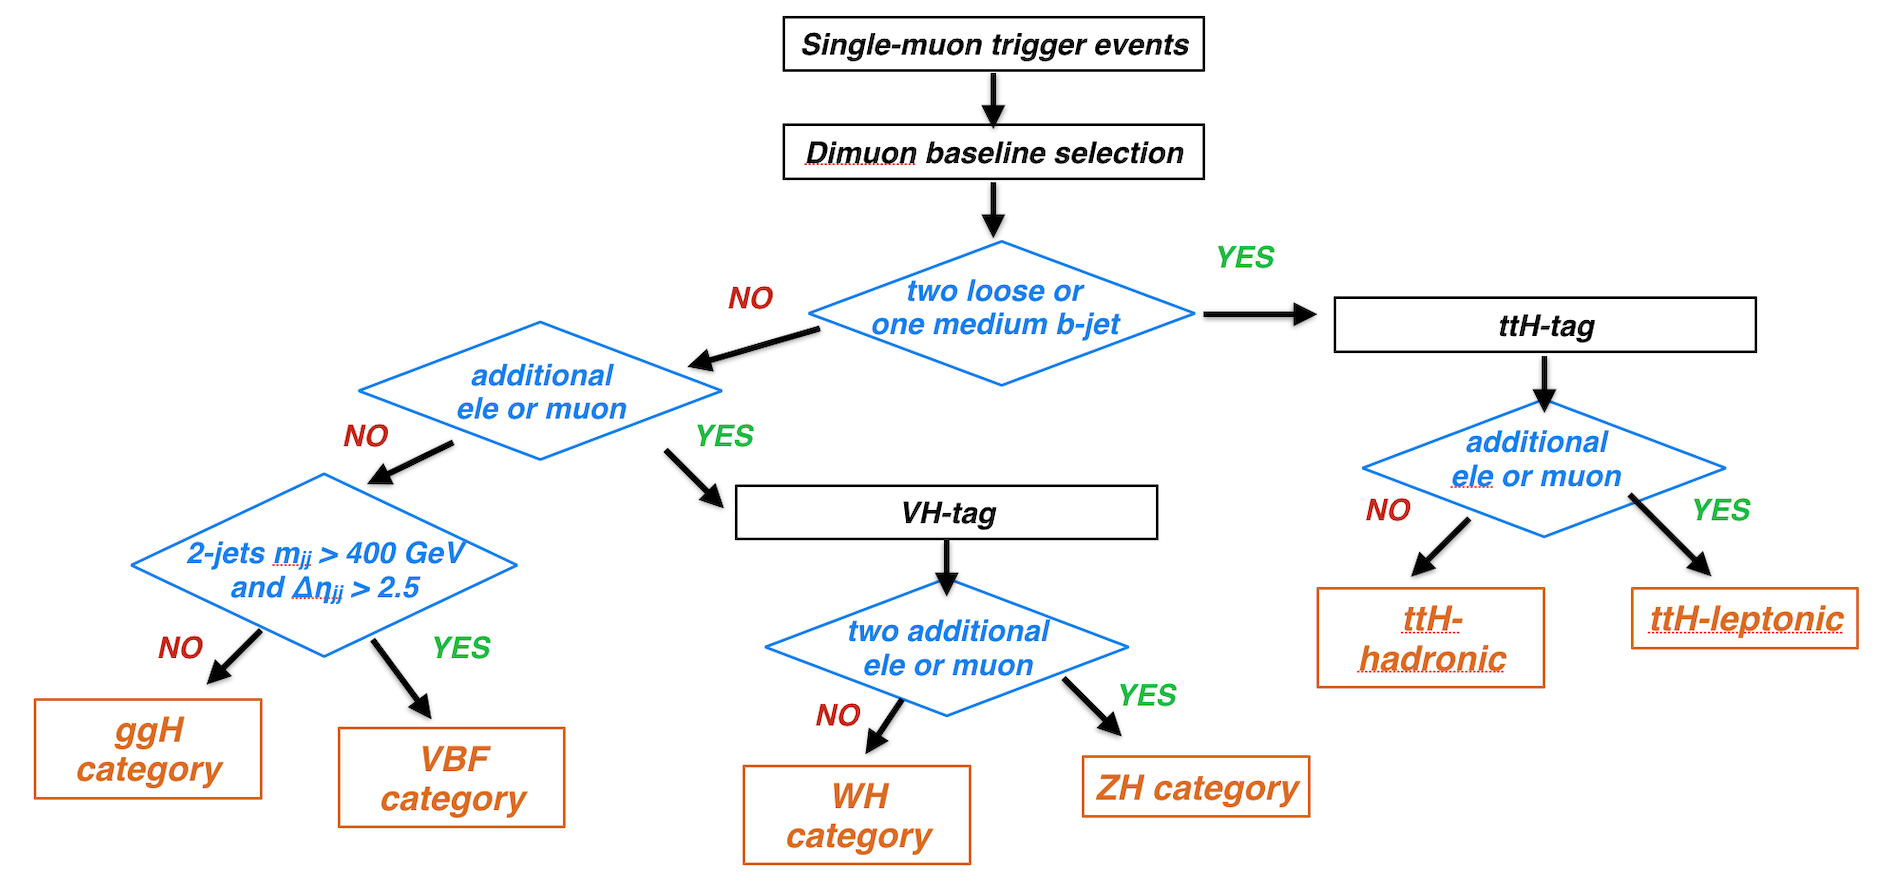
\includegraphics[width=0.9\textwidth]{pics/category_scheme.png}
    \caption{A scheme showing the procedure of assigning events to different categories. All events passing the common baseline selection
             are divided into four mutally exclusive categories: \ggH, \qqH, \VH (\WH and \ZH), and \ttH (leptonic and hadronic).}
    \label{fig:event_categories}
\end{figure}

The analysis is performed independently in each event categories. 
Given the distinct difference in the expect signal yield, the signal purity, and the background composition in different categories, 
the optimal approach are also different.
As a result, two different strategies to perform the analysis are considered:

\begin{itemize}
    \item \textbf{Data-driven parametric fit to the \mmm spectrum:} 
          As is done in the previously published analyses on the earlier data~\cite{2015184, PhysRevLett.122.021801},  
          a multi-variable-analysis (MVA) method is used to profile the separation between the signal and the background processes. 
          The MVA can be either cut-based as in the Run 1 analysis~\cite{2015184}, or machine learning (ML) based as in the analysis on the 2016 data~\cite{PhysRevLett.122.021801}.
          The MVA considers the kinematic information that is uncorrelated with the \mmm, and is used to divide the events into several regions 
          with different signal-to-background-ratio (\SoB), called the MVA-categories. 
          In each MVA-category, the signal strength is evaluated from fits to the data on the \mmm spectrum in what is called the \textit{signal fit region}, for example $110<\mmm<150 \GeV$.
          Both the signal and the background are modeled by parametric functions which are carefully studied to provide a truthful description of the physics distributions. 
          The total yield of the background is unconstrained in the fit and is determined entirely by the data.
          The effects of the systematic uncertainties from various sources on either the signal yield or the signal shape are assessed and propagated to the fit result. 
          The systematic uncertainties do not affect the background estimation since it is based on the data, not the MC prediction.
    \item \textbf{MC-based template fit to the Neural Network discriminator:}
          This approach is also based on a MVA, for which a ML algorithm, Deep Neural Network (DNN), is taken.
          The DNN takes all the kinematic variables in the events \textit{includeing the \mmm}, and profiles the discrimination between the signal and the background.
          Without making further categories, the binned template of the DNN output in the whole phasespace is used for the signal strength evaluation.
          Since the fit happens to the DNN output rather than the \mmm distribution, the \textit{signal fit region} is further divided into two parts:
          the \textit{signal region} where $115<\mmm<135 \GeV$ and the \textit{sideband region} where $110<\mmm<115 \GeV$ or $135<\mmm<150 \GeV$.
          The data is fitted simutaneuosly in both regions with the DNN templates of the signal and the background MC. 
          The systematic uncertaintise affect both the signal and the background prediction, and are employed as either the yield or the shape variations of the templates.
          The background yield is estimated from the MC and is allowed to vary within its uncertainty in the fit, in the same manner as the other systematic uncertainties.
          The signal strength is extracted from the fit in the \textit{signal region}.
          The \textit{sideband region} does not contain any signal contribution, but is nonetheless used in the fit, to enhance the constraint on the background estimation.
\end{itemize}

These two strategies should give comparable results in the ideal case, where there are abundant statistics in both the data and the MC,
and the data is well described by the MC.
However these conditions are usually not met in realistic analyses, and one strategy may become preferable over the other.
The pp collision is a very noisy environment, making it difficult to achieve an accurate modeling of many kinematic aspects,
for example the pile-up events, the parton shower, and the production of leptons through bottom or charm quarks (nonprompt leptons).
The modeling of these features usually involves extensive work in the validation of simulated samples, and is generally associated with large systematic uncertainties.
In the scenarios where the MC does not model the data very well, or where the uncertainties from MC modeling are not much smaller than the statistical uncertainty in the data,
it is more advantageous to follow the data-driven approach.
On the other hand, if a phasespace lacks enough statistics in data but can be well described by the MC, 
it is more beneficial to perform a MC-based analysis there.

The \ggH category contains the majority of the events in the \hmm analysis, and has very low \SoB. 
In all the MVA-based sub-categories, there are abundant data that the statistical uncertainty of data is smaller than the systematic uncertainties of the background prediction from MC.
Therefore the data-driven strategy is taken in the analysis in the \ggH category.
The \qqH category is featured with a good amount of events, although much less than the \ggH category, and a good \SoB.
This makes it possible to enhance the sensitivity of the analysis by picking very high \SoB regions with the help of MVA discriminators. 
Naturally, the number of events in the high \SoB regions is very low. Therefore the MC-based strategy is used in the \qqH category.
The \VH and the \ttH categories both have very few events but high \SoB, which seem like a good playground for the MC-based approach.
However, one of the main background in the \VH and \ttH categories involves the extra lepton(s) from nonprompt sources, and lacks accurate MC modeling.
Moreover, the expected signal yield in these categories is too low that it is impractical to make MC templates with many bins.
Given the dataset used in this analysis, the data-driven method is the prefered choice in both the \VH and the \ttH categories.
Overall, the \ggH, \VH, and \ttH categories follow the data-driven strategy, while the \qqH category takes the MC-based approach.

More details of the analysis strategy can be found in the paper describing this analysis~\cite{cmscollaboration2020evidence}, recently submitted by CMS. 
The following chapters will cover the object definition and the muon corrections which are common to the whole analysis, 
then the detailed steps of the analysis in the \VH category, 
and finally the results of both the \VH category and of the combination of four categories.
